\section{Experimento 1}

\subsection{Resultados}

\begin{figure}[H]
  \centering
  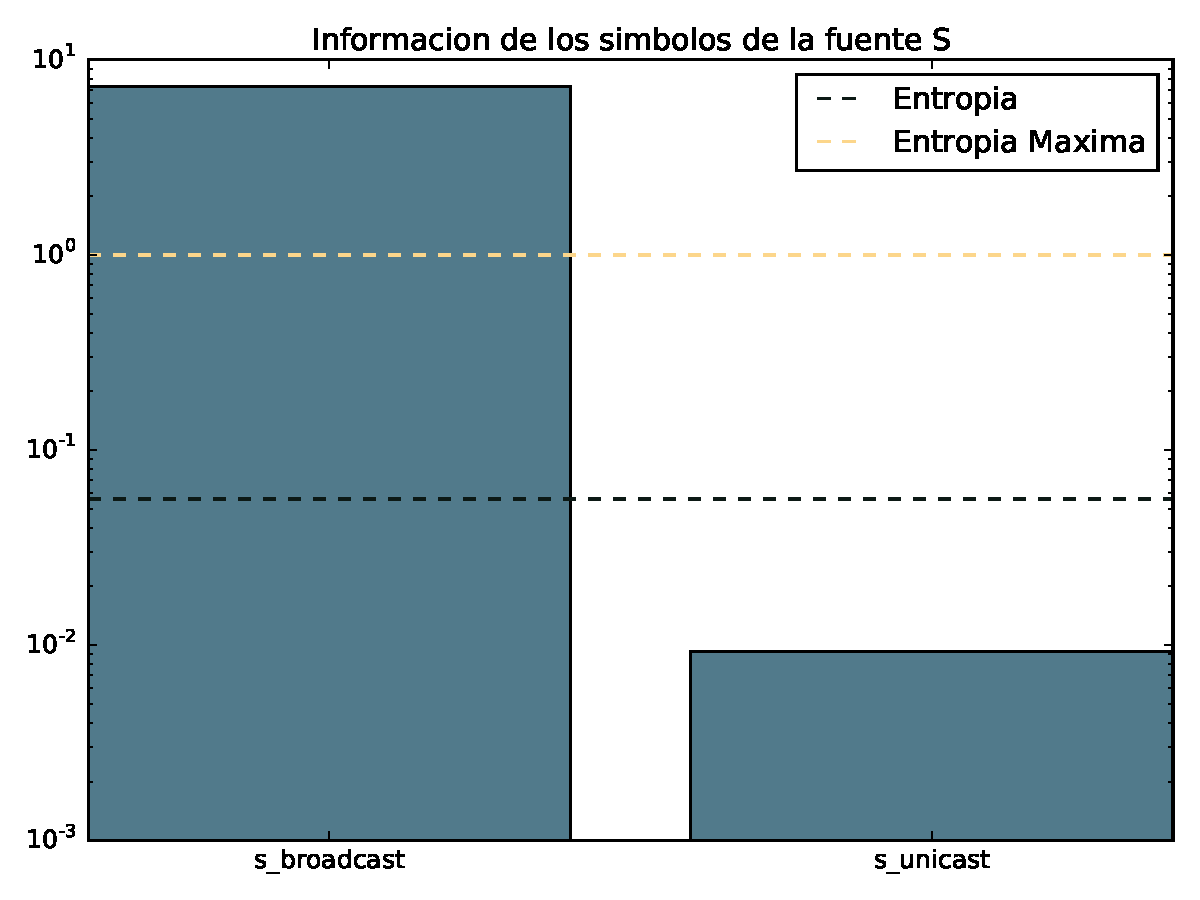
\includegraphics[width=8.5cm]{exp_starbucks/grafico1.pdf}
  \caption{\normalfont }
\end{figure}

\begin{figure}[H]
  \centering
  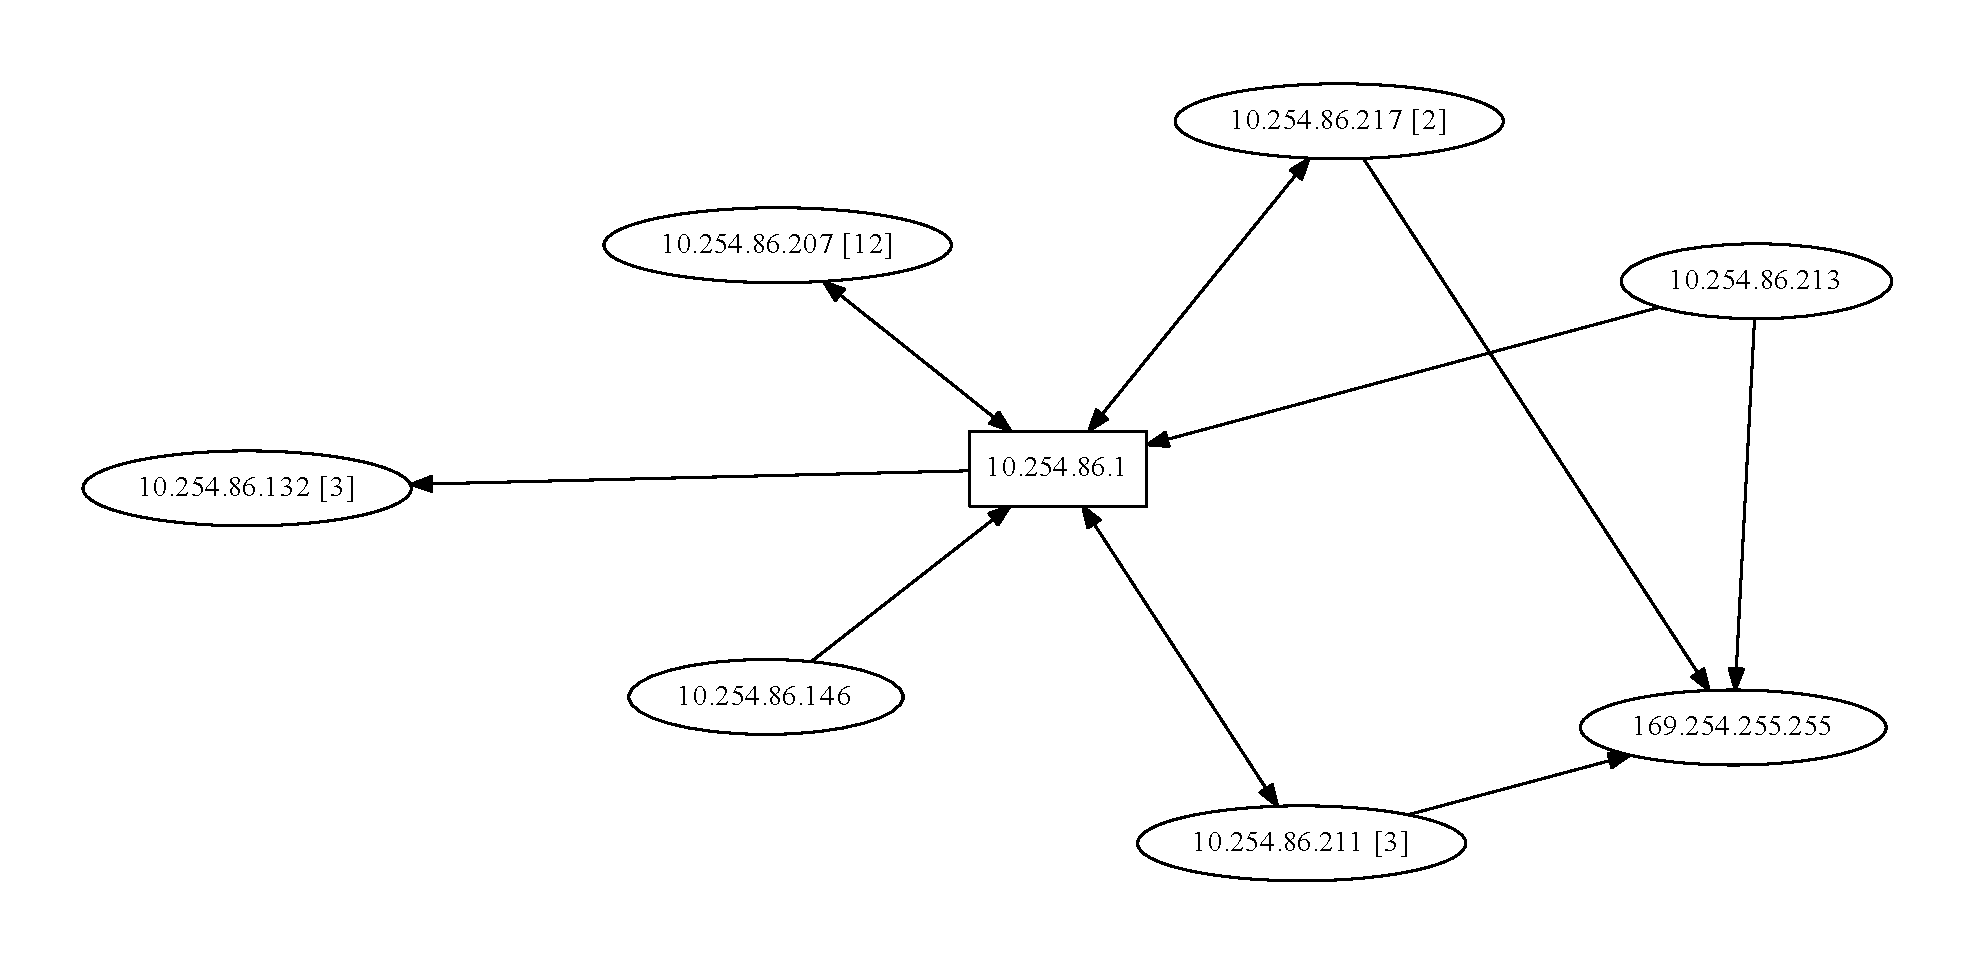
\includegraphics[width=8.5cm]{exp_starbucks/grafico2.pdf}
  \caption{  \normalfont Grafo de conectividad de la red, inferido de los paquetes who-has. Para ver con mayor detalle, se puede hacer zoom-in en el pdf. }
\end{figure}

\begin{figure}[H]
  \centering
  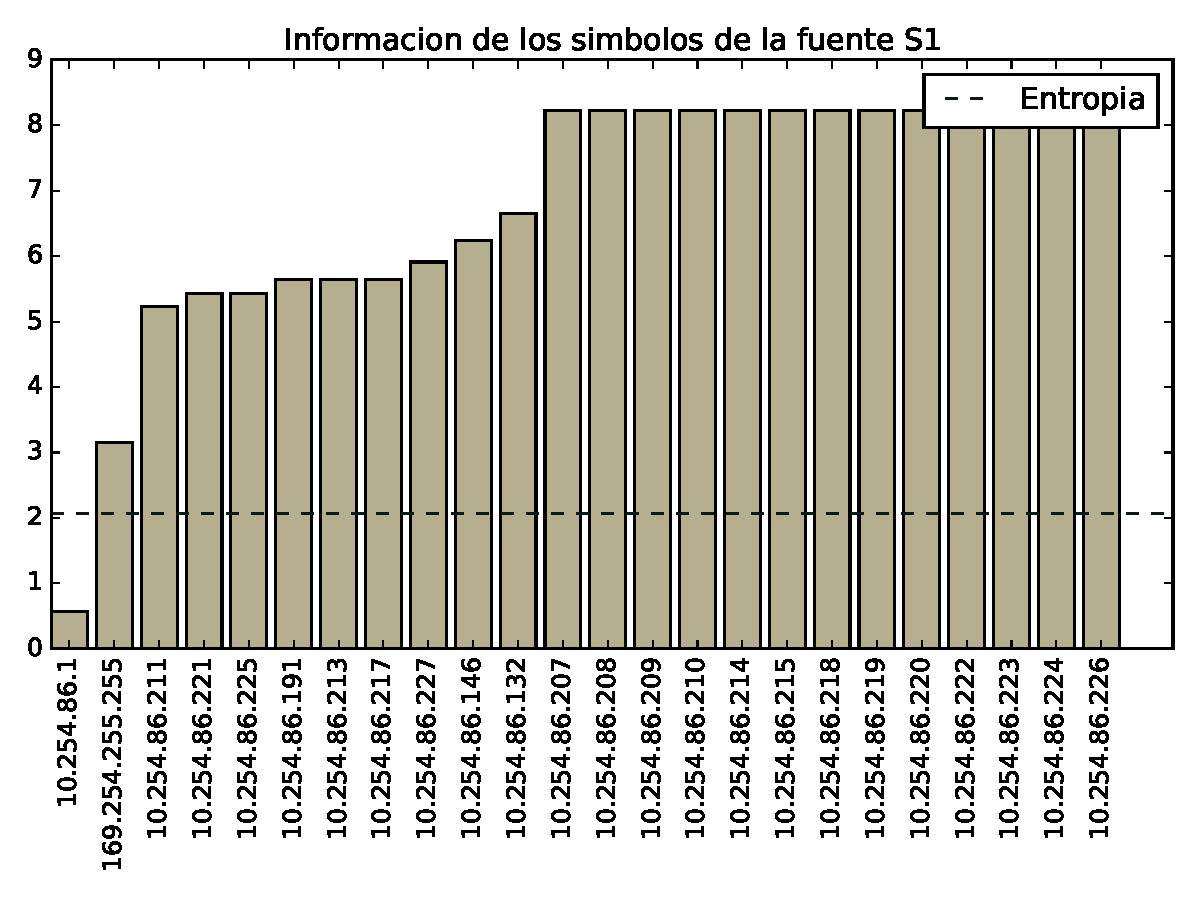
\includegraphics[width=8.5cm]{exp_starbucks/grafico3.pdf}
  \caption{ \normalfont Información de los símbolos de la fuente S1: solamente los nodos con menor información son representados.}
\end{figure}

\subsection{Discusión}

